
This chapter describes both the functional and non-functional requirements
for the various parts of the project.

\section{Functional requirements}
	
	\subsection{Social library}
	\begin{description}
		\item[Network support:] The library shall support at least two social networks.
		One is OpenSocial and the other is Facebook.
		\item[Abstractions:] The library shall provide abstractions for concepts found
		in social networks.
		\item[]
	\end{description}
	
	\subsection{Communication library}
	\begin{description}
		\item[Wireless connectivity:] Since the product will target a user-base with
		no technical background, the customer required all connections between
		devices to be wireless, so that connecting the User Interface to the Android
		mobile will be as easy as possible for the end-users. For this reason, the technical
		details of the connection should be hidden to the end-user so that the product can
		be easily operated.
		\item[Two-way communction:] The communication shall be two-way: from the
		Arduino device to Android and vice-versa.
	\end{description}


	\newpage

	\subsection{Facebook application}

	The design of the Facebook application was changed after roughly one month.

	\subsubsection{Initial design}

	\begin{description}
		\item[Login (Authentication):] The application shall handle the authentication with Facebook.
		\item[Logoff:] The user shall be able to log off once logged in.
		\item[Facebook connectivity:] The application shall be able to fetch and push data from/to Facebook.
		\item[Browsing:] The application shall let the user browse for some social content.
		\item[Sharing:] The application shall send social content to the T-Shirt application
		upon user request.
	\end{description}

	\begin{figure}[h!]
	\centering 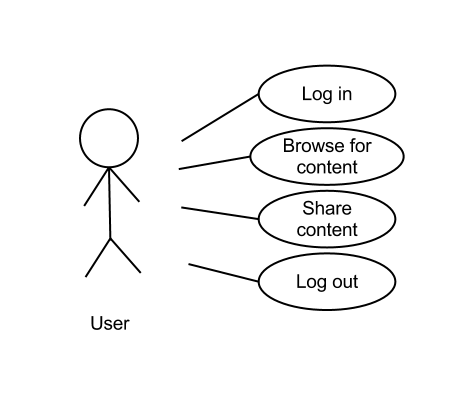
\includegraphics[scale=0.50]{img/req-socialappusecase1.png}
	\caption{Use case for the social application}
	\label{fig:req-tshirtappusecase1}
	\end{figure}

	\newpage
	
	\subsubsection{Revised design}

	\begin{description}
		\item[Login (Authentication):] The application shall handle the authentication with Facebook.
		\item[Logoff:] The user shall be able to log off once logged in.
		\item[Facebook connectivity:] The application shall fetch and push data
		from/to Facebook as requested, even when the mobile itself is idle (not operated).
		\item[User input:] Once the user is authenticated, no further user action is required.
	\end{description}
	
	\begin{figure}[h!]
	\centering 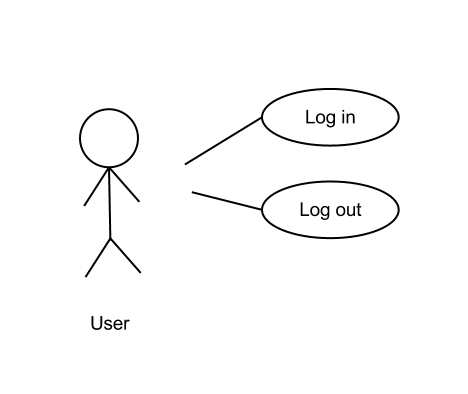
\includegraphics[scale=0.50]{img/req-socialappusecase2.png}
	\caption{Use case for the social application}
	\label{fig:req-tshirtappusecase2}
	\end{figure}

	\newpage

	\subsection{T-Shirt prototype}

	During our meeting with the customer we tried to identify the
	use cases for the T-Shirt prototype in order to have clear the requirements.

	Initially we misunderstood the use cases and proceeded with a design of
	the prototype, and consequently of the T-Shirt and Facebook application,
	which satisfied different requirements.

	The design was revised after roughly one month. See Design chapter.
	
	\begin{description}
		\item[Features:] The prototype shall map some social content
		to various embedded electronic devices.
		\item[Libraries:] The prototype shall use both the Social and
		Communication libraries.
		\item[User input:] Once the rules for the T-Shirt are set,
		no further user input shall be required.
	\end{description}

	\begin{figure}[h!]
	\centering 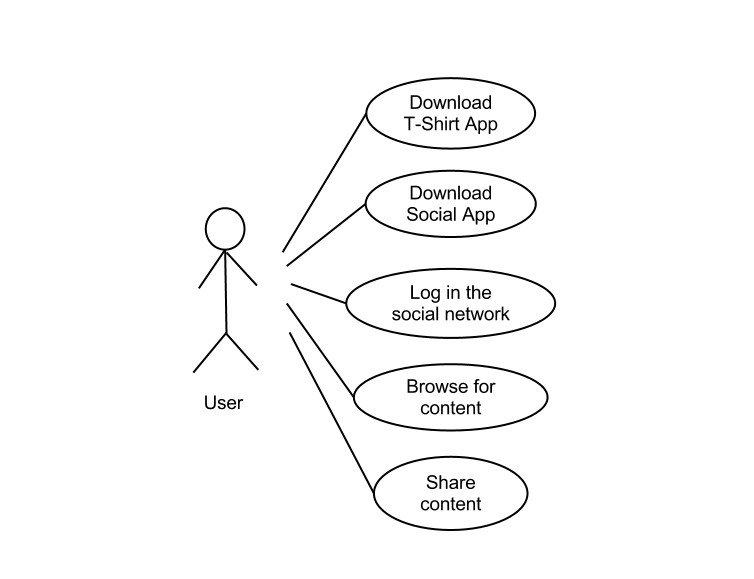
\includegraphics[scale=0.50]{img/req-usecase1.png}
	\caption{Use case for the first T-Shirt prototype's design}
	\label{fig:req-usecase1}
	\end{figure}

	\begin{figure}[h!]
	\centering 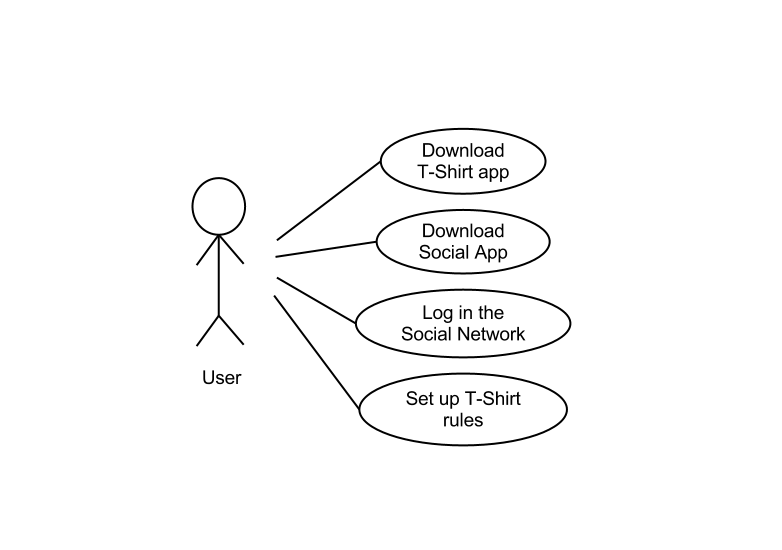
\includegraphics[scale=0.50]{img/req-usecase2.png}
	\caption{Use case for the second T-Shirt prototype's design}
	\label{fig:req-usecase2}
	\end{figure}

	\newpage

	\subsection{T-Shirt application}

	Being closely related to the T-Shirt prototype, the T-Shirt application
	also had to pursue a different design than the original one.
	
	\begin{description}
		\item[On and Off:] The user shall be able to turn the application On and Off.
		When the application is not running, no social data will be forwarded
		to the T-Shirt prototype.
		\item[Rules:] The application shall let the user setup a set of rules
		to control the behavior of the T-Shirt. Rules can be created and deleted.
		\item[User interaction:] The application shall continue to work
		when the mobile itself is idle.
	\end{description}

	\begin{figure}[h!]
	\centering 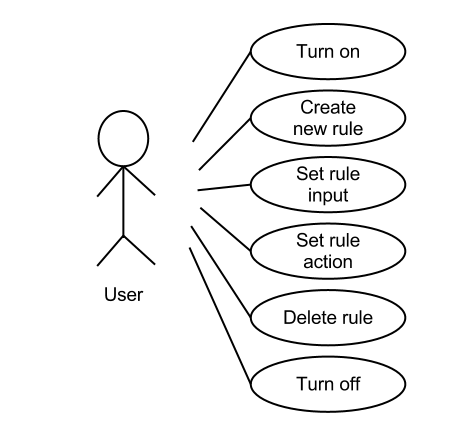
\includegraphics[scale=0.50]{img/req-tshirtappusecase.png}
	\caption{Use case for the T-Shirt application}
	\label{fig:req-tshirtappusecase}
	\end{figure}

	\newpage

	\subsection{Temperature prototype}
	\begin{description}
		\item[Features:] The prototype shall read the temperature
		using an Arduino sensor and push it to Facebook.
		\item[Libraries:] The prototype shall use both the Social and
		Communication libraries.
		\item[]
	\end{description}
	
	\subsection{Image to LED matrix prototype}
	\begin{description}
		\item[Features:] The prototype shall display an image sent by a Android
		mobile using some LEDs.
		\item[Libraries:] The prototype shall use the Communication library.
		\item[]
	\end{description}



\section{Non functional requirements}

\subsection{Libraries}

Both libraries share some non functional requirements.
For the sake of simplicity they will be listed together.

\begin{description}
	\item[Extensibility:] The library shall have a modular design
	in order to be easily extended. The software that will be developed for
	this project will serve as a proof-of-concept and possibily as a starting point
	for other research projects. For this reason a flexible, modular software
	architecture is an important requirement for our customer. The code shall be
	developed in independent, thus reusable modules so that adding new functionality
	will be fairly easy for new developers.
	\item[Target platform:] The library shall be compatible with the Android
	system starting from version 2.2. This will place restrictions on the software
	and on the programming languages that will be adopted.
	\item[Documentation:] The library shall be documented using Javadoc.
	Since the product is going to be further developed by other people and is
	mainly designed for easier application development then proper research and usage
	documentation is important. Proper documentation or tutorials should describe how
	the end-user can easily use the libraries without any technical knowledge of how
	the library works.
	\item[Licensing:] The library shall be released under the Apache License 2.0.
	The customer made clear that all the software developed needs to be released
	under a permissive, Apache software license. This implies that pre-existing
	software that will eventually be adopted and incorporated in the project must
	have a compatible license.
\end{description}


\subsection{Prototypes}

Non-functional prototypes' requirements.


\subsection{Applications}

All the applications share some non functional requirements.
For the sake of simplicity they will be listed below:

\begin{description}
	\item[Target platform:] The applications shall be compatible with the Android
	system starting from version 2.2. This will place restrictions on the software
	and on the programming languages that will be adopted.
	\item[Documentation:] The applications shall be documented using Javadoc.
	\item[Licensing:] The applications shall be released under the Apache License 2.0.
\end{description}

\newpage

\section{Functional Requirements}

\todo{
	remove? it has been written somewhere else
	in a more structured way.
}

Requirements are ordered by importance.

\begin{itemize}
\item{F1: Communication Library}\newline
The Android should use the Communication Library to connect wirelessly 
to an Arduino module and establish two way communication.

\item{F2: Social Library}\newline
Android applications should be able to retrieve social data from any 
supported social network through the use of the Social Library. General 
concepts applicable in any social network such as Person, Group, Message, etc.
should be extracted and devised into a model interface that is easy for the application
developer to use.

\item{F3: Wireless connectivity}\newline
Since the product will target a user-base with no technical background,
the customer required all connections between devices to be wireless,
so that connecting the User Interface to the Android mobile will be
as easy as possible for the end-users. For this reason, the technical
details of the connection should be hidden to the end-user so that
the product can be easily operated.
	
\item{F4: Prototype}\newline
To show that the concept of Tangible User Interfaces for Android applications
(including social networks) using Arduino is not only possible, but
also a feasible market product, the customer is interested in a working
prototype. Develop three prototypes, one more complex prototype showcasing the 
functionality of both the Communication Library and Social Library. The other
two prototypes should be much simpler in complexity and their purpose is just to
prove that the libraries can be successfully used for different prototypes.

\item{F5: Support Android platform 2.2}\newline
The library should be compatible with Android API version 2.2 and later. This is to
ensure that any application built with our library is compatible with as many Android
versions as possible. The specific version to be supported was set by the customer.
\end{itemize}


%Non functional Requirements
\section{Non-functional Requirements}

\begin{itemize}
\item{NF1: Flexible software architecture}\newline
The software that will be developed for this project will serve as
a proof-of-concept and possibily as a starting point for other research
projects. For this reason a flexible, modular software architecture
is an important requirement for our customer. The code shall be developed
in independent, thus reusable modules so that adding new functionality
will be fairly easy for new developers.

\item{NF2: Software licenses}\newline
The customer made clear that the software developed needs to be released
under a permissive, Apache compatible software license. This implies
that pre-existing software that will eventually be adopted and incorporated
in the project must have a compatible license.

\item{NF3: API Documentation and Javadoc}\newline
Since the product is going to be further developed by other people and is
mainly designed for easier application development then proper research and usage
documentation is important. Proper documentation or tutorials should describe how
the end-user can easily use the libraries without any technical knowledge of how
the library works.

\item{NF4: Target platforms}\newline
The product has to target the Android platform and Arduino.
This will place restrictions on the software and on the programming languages that will be adopted.
\end{itemize}

\newpage
\section{Use cases}
\todo{
	review.
}
Use Case:
We have two actors we are working with. One is the developer creating the application using our framework.
The other one is the end user with the final product. We are not directly working with the end user as an actor,
but we still want to make our framework so it is simple for developer to have a product with an easy connection to the arduino board.

Our focus on the actor developer is centered around the software he create. We do not know, and we don't need to
know what product he is making. We will work on two parts he can to implement in his software. It will be the setup and
transfer protocol to arduino and Intents to send and recive updates from social services.

For the end user, we want the setup to connect his phone to the developer to be as easy as possible. The focus will be on
simplified connection to arduino board, and easy connection to social services from application.

\todo{
	outdated?
}
\begin{figure}[hb!]
\centering 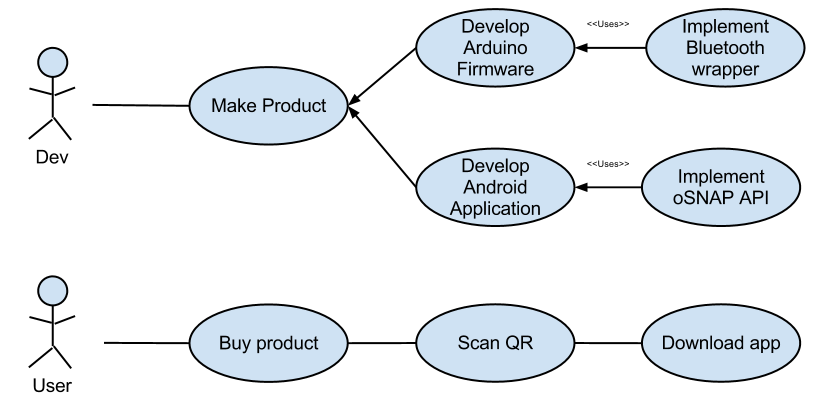
\includegraphics[scale=0.50]{img/use-cases.png}
\caption{Use cases}
\label{fig:architecture-usecases}
\end{figure}